% Options for packages loaded elsewhere
\PassOptionsToPackage{unicode}{hyperref}
\PassOptionsToPackage{hyphens}{url}
%
\documentclass[
]{article}
\usepackage{lmodern}
\usepackage{amssymb,amsmath}
\usepackage{ifxetex,ifluatex}
\ifnum 0\ifxetex 1\fi\ifluatex 1\fi=0 % if pdftex
  \usepackage[T1]{fontenc}
  \usepackage[utf8]{inputenc}
  \usepackage{textcomp} % provide euro and other symbols
\else % if luatex or xetex
  \usepackage{unicode-math}
  \defaultfontfeatures{Scale=MatchLowercase}
  \defaultfontfeatures[\rmfamily]{Ligatures=TeX,Scale=1}
\fi
% Use upquote if available, for straight quotes in verbatim environments
\IfFileExists{upquote.sty}{\usepackage{upquote}}{}
\IfFileExists{microtype.sty}{% use microtype if available
  \usepackage[]{microtype}
  \UseMicrotypeSet[protrusion]{basicmath} % disable protrusion for tt fonts
}{}
\makeatletter
\@ifundefined{KOMAClassName}{% if non-KOMA class
  \IfFileExists{parskip.sty}{%
    \usepackage{parskip}
  }{% else
    \setlength{\parindent}{0pt}
    \setlength{\parskip}{6pt plus 2pt minus 1pt}}
}{% if KOMA class
  \KOMAoptions{parskip=half}}
\makeatother
\usepackage{xcolor}
\IfFileExists{xurl.sty}{\usepackage{xurl}}{} % add URL line breaks if available
\IfFileExists{bookmark.sty}{\usepackage{bookmark}}{\usepackage{hyperref}}
\hypersetup{
  hidelinks,
  pdfcreator={LaTeX via pandoc}}
\urlstyle{same} % disable monospaced font for URLs
\usepackage[margin=1in]{geometry}
\usepackage{color}
\usepackage{fancyvrb}
\newcommand{\VerbBar}{|}
\newcommand{\VERB}{\Verb[commandchars=\\\{\}]}
\DefineVerbatimEnvironment{Highlighting}{Verbatim}{commandchars=\\\{\}}
% Add ',fontsize=\small' for more characters per line
\usepackage{framed}
\definecolor{shadecolor}{RGB}{248,248,248}
\newenvironment{Shaded}{\begin{snugshade}}{\end{snugshade}}
\newcommand{\AlertTok}[1]{\textcolor[rgb]{0.94,0.16,0.16}{#1}}
\newcommand{\AnnotationTok}[1]{\textcolor[rgb]{0.56,0.35,0.01}{\textbf{\textit{#1}}}}
\newcommand{\AttributeTok}[1]{\textcolor[rgb]{0.77,0.63,0.00}{#1}}
\newcommand{\BaseNTok}[1]{\textcolor[rgb]{0.00,0.00,0.81}{#1}}
\newcommand{\BuiltInTok}[1]{#1}
\newcommand{\CharTok}[1]{\textcolor[rgb]{0.31,0.60,0.02}{#1}}
\newcommand{\CommentTok}[1]{\textcolor[rgb]{0.56,0.35,0.01}{\textit{#1}}}
\newcommand{\CommentVarTok}[1]{\textcolor[rgb]{0.56,0.35,0.01}{\textbf{\textit{#1}}}}
\newcommand{\ConstantTok}[1]{\textcolor[rgb]{0.00,0.00,0.00}{#1}}
\newcommand{\ControlFlowTok}[1]{\textcolor[rgb]{0.13,0.29,0.53}{\textbf{#1}}}
\newcommand{\DataTypeTok}[1]{\textcolor[rgb]{0.13,0.29,0.53}{#1}}
\newcommand{\DecValTok}[1]{\textcolor[rgb]{0.00,0.00,0.81}{#1}}
\newcommand{\DocumentationTok}[1]{\textcolor[rgb]{0.56,0.35,0.01}{\textbf{\textit{#1}}}}
\newcommand{\ErrorTok}[1]{\textcolor[rgb]{0.64,0.00,0.00}{\textbf{#1}}}
\newcommand{\ExtensionTok}[1]{#1}
\newcommand{\FloatTok}[1]{\textcolor[rgb]{0.00,0.00,0.81}{#1}}
\newcommand{\FunctionTok}[1]{\textcolor[rgb]{0.00,0.00,0.00}{#1}}
\newcommand{\ImportTok}[1]{#1}
\newcommand{\InformationTok}[1]{\textcolor[rgb]{0.56,0.35,0.01}{\textbf{\textit{#1}}}}
\newcommand{\KeywordTok}[1]{\textcolor[rgb]{0.13,0.29,0.53}{\textbf{#1}}}
\newcommand{\NormalTok}[1]{#1}
\newcommand{\OperatorTok}[1]{\textcolor[rgb]{0.81,0.36,0.00}{\textbf{#1}}}
\newcommand{\OtherTok}[1]{\textcolor[rgb]{0.56,0.35,0.01}{#1}}
\newcommand{\PreprocessorTok}[1]{\textcolor[rgb]{0.56,0.35,0.01}{\textit{#1}}}
\newcommand{\RegionMarkerTok}[1]{#1}
\newcommand{\SpecialCharTok}[1]{\textcolor[rgb]{0.00,0.00,0.00}{#1}}
\newcommand{\SpecialStringTok}[1]{\textcolor[rgb]{0.31,0.60,0.02}{#1}}
\newcommand{\StringTok}[1]{\textcolor[rgb]{0.31,0.60,0.02}{#1}}
\newcommand{\VariableTok}[1]{\textcolor[rgb]{0.00,0.00,0.00}{#1}}
\newcommand{\VerbatimStringTok}[1]{\textcolor[rgb]{0.31,0.60,0.02}{#1}}
\newcommand{\WarningTok}[1]{\textcolor[rgb]{0.56,0.35,0.01}{\textbf{\textit{#1}}}}
\usepackage{graphicx,grffile}
\makeatletter
\def\maxwidth{\ifdim\Gin@nat@width>\linewidth\linewidth\else\Gin@nat@width\fi}
\def\maxheight{\ifdim\Gin@nat@height>\textheight\textheight\else\Gin@nat@height\fi}
\makeatother
% Scale images if necessary, so that they will not overflow the page
% margins by default, and it is still possible to overwrite the defaults
% using explicit options in \includegraphics[width, height, ...]{}
\setkeys{Gin}{width=\maxwidth,height=\maxheight,keepaspectratio}
% Set default figure placement to htbp
\makeatletter
\def\fps@figure{htbp}
\makeatother
\setlength{\emergencystretch}{3em} % prevent overfull lines
\providecommand{\tightlist}{%
  \setlength{\itemsep}{0pt}\setlength{\parskip}{0pt}}
\setcounter{secnumdepth}{-\maxdimen} % remove section numbering

\author{}
\date{\vspace{-2.5em}}

\begin{document}

\hypertarget{lreputah}{%
\section{LREPUtah}\label{lreputah}}

\href{https://travis-ci.com/jiqiaingwu/LREPUtah}{\includegraphics{https://travis-ci.com/jiqiaingwu/LREPUtah.svg?branch=main}}
\href{https://github.com/jiqiaingwu/LREPUtah/actions}{\includegraphics{https://github.com/jiqiaingwu/LREPUtah/workflows/R-CMD-check/badge.svg}}

The goal of LREPUtah is to estimate the Parameters for the Pareto
Distribution and test Pareto vs.~Exponential Distributions

\hypertarget{installation}{%
\subsection{Installation}\label{installation}}

You can install the released version of LREPUtah from
\href{https://CRAN.R-project.org}{CRAN} with:

\begin{Shaded}
\begin{Highlighting}[]
\KeywordTok{install.packages}\NormalTok{(}\StringTok{"LREPUtah"}\NormalTok{)}
\end{Highlighting}
\end{Shaded}

And the development version from \href{https://github.com/}{GitHub}
with:

\begin{Shaded}
\begin{Highlighting}[]
\CommentTok{# install.packages("devtools")}
\NormalTok{devtools}\OperatorTok{::}\KeywordTok{install_github}\NormalTok{(}\StringTok{"jiqiaingwu/LREPUtah"}\NormalTok{)}
\end{Highlighting}
\end{Shaded}

\hypertarget{introduction}{%
\subsection{Introduction}\label{introduction}}

Our test is a likelihood ratio test of the following hypotheses:

Ho: data comes from an exponential distribution, versus the alternative

H1: data comes from a Pareto distribution.

The approach is to consider the ratio of the maxima of the likelihoods
of the observed sample under the Pareto or exponential (in the
numerator) and exponential (in the denominator) models. The logarithm
(natural) of the likelihood ratio, the L statistic, is:

\begin{figure}
\centering
\includegraphics{https://latex.codecogs.com/svg.image?L=log\%5Cfrac\%7Bmax(\%5Cunderset\%7B\%5Calpha\%20\%3E0,s\%3E0\%7D\%7Bsup\%7DL_\%7BPareto\%7D(\%5Cvec\%7Bx\%7D\%7C\%5Calpha,s),\%5Cunderset\%7B\%5Csigma\%20\%3E0\%7D\%7Bsup\%7DL_\%7Bexp\%7D(\%5Cvec\%7Bx\%7D\%20\%7C\%20\%5Csigma\%20))\%7D\%7B\%5Cunderset\%7B\%5Csigma\%20\%3E0\%7D\%7Bsup\%7DL_\%7Bexp\%7D(\%5Cvec\%7Bx\%7D\%7C\%5Csigma\%20)\%7D}
\caption{main equation}
\end{figure}

Where
\includegraphics{https://latex.codecogs.com/svg.image?\%5Cvec\%7Bx\%7D}
is the observed sample of excesses and
\includegraphics{https://latex.codecogs.com/svg.image?L_\%7BPareto\%7D(\%5Cvec\%7Bx\%7D\%7C\%5Calpha\%20,s)}
and
\includegraphics{https://latex.codecogs.com/svg.image?L_\%7Bexp\%7D(\%5Cvec\%7Bx\%7D\%7C\%5Csigma\%20)}
are the likelihood functions of the sample under Pareto and exponential
models, respectively.

We use a Pareto distribution with the survival function
\includegraphics{https://latex.codecogs.com/svg.image?S(x)=P(X\%3Ex)=(\%5Cfrac\%7B1\%7D\%7B1+\%5Cfrac\%7Bx\%7D\%7Bs\%5Calpha\%7D\%7D)\%5E\%7Ba\%7D}
and exponential distribution with the survival function
\includegraphics{https://latex.codecogs.com/svg.image?S(x)=P(X\%3Ex)=exp(-\%20\%5Cfrac\%7Bx\%7D\%7B\%5Csigma\%20\%7D)}.
To compute L, both likelihoods are maximized first (via maximum
likelihood estimates, MLEs, of the parameters), and then the natural
logarithm of their ratio is taken as the likelihood ratio statistic.
Panorska et al.~(2007) provide the necessary theoretical results for the
implementation of the numerical routines necessary for the computation
of L. The properties of the test, proofs and more details on the
optimization process appear separately in Kozubowski et al.(2007)

The (1-γ)100 percentiles of L provide the critical numbers for our test
on the significance level γ. The test is one-sided and we reject the
null hypothesis if the computed value of the test statistic exceeds the
critical number. We have computed some common percentiles for the
distribution of L under the null hypothesis for different sample sizes
and for the limiting case. The percentiles for finite sample sizes were
computed via Monte Carlo simulation with 10,000 samples of a given size
from the exponential distribution (Table below).

\begin{figure}
\centering
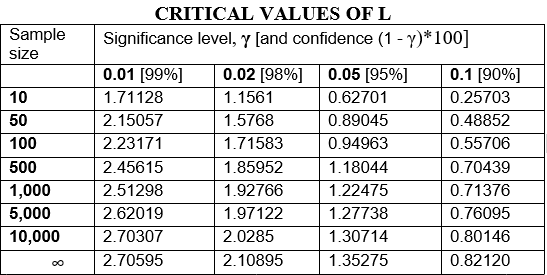
\includegraphics{man/figures/Table1.PNG}
\caption{Table 1}
\end{figure}

\hypertarget{example}{%
\subsection{Example}\label{example}}

This is a basic example which shows you how to solve a common problem:

\begin{Shaded}
\begin{Highlighting}[]
\KeywordTok{library}\NormalTok{(LREPUtah)}

\CommentTok{###example when data is Exponential}
\CommentTok{####################################}

\NormalTok{x<-}\KeywordTok{rexp}\NormalTok{(}\DecValTok{1000}\NormalTok{,}\FloatTok{0.000000000005}\NormalTok{)}
\DecValTok{1}\OperatorTok{/}\KeywordTok{mean}\NormalTok{(x)}
\CommentTok{#> [1] 5.06287e-12}
\KeywordTok{sigmaalphaLREP}\NormalTok{(x,}\DecValTok{10}\OperatorTok{^-}\DecValTok{12}\NormalTok{)}
\CommentTok{#>         s.hat     a.hat log.like.ratio}
\CommentTok{#> [1,] 85323308 0.1396723              0}
\KeywordTok{expparetotest}\NormalTok{(x,}\FloatTok{0.05}\NormalTok{)}
\CommentTok{#>         s.hat     a.hat log.like.ratio}
\CommentTok{#> [1,] 85323308 0.1396723              0}
\CommentTok{#> Critical value: 2.446109 }
\CommentTok{#> Deviance statistic: 0 }
\CommentTok{#> Data is comming from an exponential distribution}

\CommentTok{##asymptotic p-value}
\DecValTok{1}\OperatorTok{/}\DecValTok{2}\OperatorTok{*}\NormalTok{(}\DecValTok{1}\OperatorTok{-}\KeywordTok{pchisq}\NormalTok{(}\DecValTok{0}\NormalTok{,}\DataTypeTok{df=}\DecValTok{1}\NormalTok{))}
\CommentTok{#> [1] 0.5}


\NormalTok{x<-}\KeywordTok{rexp}\NormalTok{(}\DecValTok{1000}\NormalTok{,}\FloatTok{0.1}\NormalTok{)}
\DecValTok{1}\OperatorTok{/}\KeywordTok{mean}\NormalTok{(x)}
\CommentTok{#> [1] 0.09671063}
\KeywordTok{sigmaalphaLREP}\NormalTok{(x,}\DecValTok{10}\OperatorTok{^-}\DecValTok{12}\NormalTok{)}
\CommentTok{#>         s.hat    a.hat log.like.ratio}
\CommentTok{#> [1,] 16554.27 1601.956              0}
\KeywordTok{expparetotest}\NormalTok{(x,}\FloatTok{0.05}\NormalTok{)}
\CommentTok{#>         s.hat    a.hat log.like.ratio}
\CommentTok{#> [1,] 16554.27 1601.956              0}
\CommentTok{#> Critical value: 2.446109 }
\CommentTok{#> Deviance statistic: 0 }
\CommentTok{#> Data is comming from an exponential distribution}

\CommentTok{##asymptotic p-value}
\DecValTok{1}\OperatorTok{/}\DecValTok{2}\OperatorTok{*}\NormalTok{(}\DecValTok{1}\OperatorTok{-}\KeywordTok{pchisq}\NormalTok{(}\FloatTok{1.596044}\NormalTok{,}\DataTypeTok{df=}\DecValTok{1}\NormalTok{))}
\CommentTok{#> [1] 0.1032324}


\CommentTok{###example when data is Pareto}
\CommentTok{####################################}
\NormalTok{pareto.generation<-}\StringTok{ }\ControlFlowTok{function}\NormalTok{(s,a,n)}
\NormalTok{\{}
\NormalTok{    u<-}\KeywordTok{runif}\NormalTok{(n)}
\NormalTok{    x<-s}\OperatorTok{*}\NormalTok{((}\DecValTok{1}\OperatorTok{-}\NormalTok{u)}\OperatorTok{^}\NormalTok{(}\OperatorTok{-}\DecValTok{1}\OperatorTok{/}\NormalTok{a)}\OperatorTok{-}\DecValTok{1}\NormalTok{)}
\NormalTok{    x}
\NormalTok{\}}


\NormalTok{x<-}\KeywordTok{pareto.generation}\NormalTok{(}\DecValTok{10}\NormalTok{,}\DecValTok{7}\NormalTok{,}\DecValTok{1000}\NormalTok{)}
\KeywordTok{sigmaalphaLREP}\NormalTok{(x,}\DecValTok{10}\OperatorTok{^-}\DecValTok{12}\NormalTok{)}
\CommentTok{#>         s.hat    a.hat log.like.ratio}
\CommentTok{#> [1,] 8.081202 5.840223       28.05404}
\KeywordTok{expparetotest}\NormalTok{(x,}\FloatTok{0.05}\NormalTok{)}
\CommentTok{#>         s.hat    a.hat log.like.ratio}
\CommentTok{#> [1,] 8.081202 5.840223       28.05404}
\CommentTok{#> Critical value: 2.446109 }
\CommentTok{#> Deviance statistic: 28.05404 }
\CommentTok{#> Data is comming from Pareto distribution}

\CommentTok{##asymptotic p-value}
\DecValTok{1}\OperatorTok{/}\DecValTok{2}\OperatorTok{*}\NormalTok{(}\DecValTok{1}\OperatorTok{-}\KeywordTok{pchisq}\NormalTok{(}\FloatTok{14.43144}\NormalTok{,}\DataTypeTok{df=}\DecValTok{1}\NormalTok{))}
\CommentTok{#> [1] 7.267762e-05}
\end{Highlighting}
\end{Shaded}

\end{document}
